\documentclass{oblivoir}
\usepackage{amsmath,amssymb,amsthm,kotex,mdframed,paralist,graphicx,tabu,tabto}
\newcommand\pb[1]{\ensuremath{\fbox{\phantom{#1}}}}

\usepackage{fapapersize}
\usefapapersize{210mm,297mm,40mm,40mm,30mm,30mm}

\newcounter{num}
\newcommand\prob[1]
{\par\noindent\stepcounter{num} \textbf{문제 \thenum) #1}\par\noindent}
\newcommand\ans[1]
{\par{\raggedleft\textbf{답 : #1}
\par}\bigskip}
%%%
\begin{document}

%%%
\section{수열의 극한}
%%
\subsection{정의}
(1) \(\displaystyle\lim_{n\to\infty}\left(3-\frac1n\right)\)
\tabto{0.5\textwidth}
(2) \(\displaystyle\lim_{n\to\infty}\frac{1+2+3+\cdots+n}{n^2+1}\)

%%
\subsection{기본성질}
\begin{enumerate}[(1)]
\item
\(\{a_n\}\)이 수렴하고 \(c\)가 실수이면 \(\{ca_n\}\)이 수렴한다.
\item
\(\{a_n\}\)이 수렴하고 \(\{b_n\}\)이 수렴하면 \(\{a_n+b_n\}\)이 수렴한다.
\item
\(\{a_n\}\)이 수렴하고 \(\{b_n\}\)이 수렴하면 \(\{a_nb_n\}\)이 수렴한다.
\item
\(a_n<b_n\)이고 \(\{a_n\}\), \(\{b_n\}\)이 수렴하면 \(\displaystyle\lim_{n\to\infty}a_n\)\:\:\pb{\(\le\)}\:\:\(\displaystyle\lim_{n\to\infty}b_n\)이다.
\item
\(\{a_n+b_n\}\), \(\{a_n-b_n\}\)이 각각 수렴하면 \(\{a_n\}\), \(\{b_n\}\)도 수렴한다. (T, F)
\item
\(\displaystyle\lim_{n\to\infty}a_nb_n=0\)이면 \(\displaystyle\lim_{n\to\infty}a_n=0\) 또는 \(\displaystyle\lim_{n\to\infty}b_n=0\)이다. (T, F)
\item
\(\displaystyle\lim_{n\to\infty}{a_n}^2=\alpha^2\)이면 \(\displaystyle\lim_{n\to\infty}a_n=\alpha\) 또는 \(\displaystyle\lim_{n\to\infty}a_n=-\alpha\)이다. (T, F)
\item
\(a_{n+1}=\sqrt{a_n}\)이면 \(\displaystyle\lim_{n\to\infty}a_n=\pb0\)이다.
\end{enumerate}

%%%
\section{함수의 극한}
%%
\subsection{정의}
(1) \(\displaystyle\lim_{x\to3}f(x)\)가 존재한다. \(\iff\) \(\displaystyle\lim_{\pb{aaa}}f(x)=\displaystyle\lim_{\pb{aaa}}f(x)\)

\bigskip\noindent
(2) \(\displaystyle\lim_{x\to-1}(x+3)\)
\tabto{0.5\textwidth}
(3) \(\displaystyle\lim_{x\to0+}\frac1x\)

%%
\subsection{기본성질}
\begin{enumerate}[(1)]
\item
\(\displaystyle\lim_{x\to2}f(x)\)가 존재하고 \(\displaystyle\lim_{x\to2}g(x)\)가 존재하면 \(\displaystyle\lim_{x\to2}\left(f(x)-g(x)\right)\)가 존재한다.
\item
\(\displaystyle\lim_{x\to\infty}f(x)\)가 존재하고 \(\displaystyle\lim_{x\to\infty}g(x)\)가 존재하면 \(\displaystyle\lim_{x\to\infty}\frac{f(x)}{g(x)}\)가 존재한다.
\(\left(단,\:\:\pb{\(\displaystyle\lim_{x\to\infty}\frac g(x)\neq0\)}\right)\)
\item
\(f(x)<g(x)\)이고 \(\displaystyle\lim_{x\to4}f(x)\), \(\displaystyle\lim_{x\to4}g(x)\)가 존재하면 \(\displaystyle\lim_{x\to4}f(x)\)\:\:\pb{\(\le\)}\:\:\(\displaystyle\lim_{x\to4}g(x)\)이다.
\item
\(\displaystyle\lim_{x\to a}f(x)\)와 \(\displaystyle\lim_{x\to a}f(x)g(x)\)의 값이 존재하면 \(\displaystyle\lim_{x\to a}g(x)\)의 값도 존재한다. (T, F)
\item
\(\displaystyle\lim_{x\to a}f(x)\)와 \(\displaystyle\lim_{x\to a}\frac{g(x)}{f(x)}\)의 값이 존재하면 \(\displaystyle\lim_{x\to a}g(x)\)의 값도 존재한다. (T, F)
\end{enumerate}

%%%
\section{함수의 연속}

%%
\subsection{정의}
(1) 함수 \(f(x)\)가 \(x=3\)에서 연속이다. \(\iff\) \(\pb{\(\displaystyle\lim_{x\to3}f(x)\)}=\pb{f(3)}\)
\
(2) 함수 \(f(x)=|x-1|\)는 \(x=1\)에서 연속이다. (T, F)
\\
(3) 함수 \(f(x)=|x|\)는 \(x=1\)에서 연속이다. (T, F)
\\
(4) 최대\(\cdot\)최소의 정리 : 함수 \(f(x)\)가 \(\big(\) 열린구간 \((a,b)\) / 닫힌구간 \([a,b]\) \(\big)\)에서 ( 연속 / 불연속 )이면 최댓값과 최솟값을 가진다.
\\
(5) 사이값 정리 :
함수 \(f(x)\)가 연속이고, \(f(1)=5\), \(f(4)=2\)일 때, \(f(c)=3\)을 만족시키는 실수 \(c\)가 존재한다.
(단, \(\pb1<c<\pb4\))

%%
\subsection{기본성질}
\begin{enumerate}[(1)]
\item
\(f(x)\)가 \(x=a\)에서 연속이고 \(g(x)\)도 \(x=a\)에서 연속이면 함수 \(f(x)+g(x)\)도 \(x=a\)에서 연속이다.
\item
모든 다항함수는 연속이다. (T, F)
\item
\(f(x)\)가 \(x=a\)에서 연속이고 \(g(x)\)가 \(x=f(a)\)에서 연속이면 함수 \((g\circ f)(x)\)도 \(x=a\)에서 연속이다.
\end{enumerate}

\newpage
%%%
\section{문제들}

%%
%\prob{}
%\(\displaystyle\lim_{n\to\infty}\sqrt n\left(\sqrt{n+1}-\sqrt{n-1}\right)\)의 값은?
%\ans{\(1\)}
%
%%
%\prob{}
%\(\displaystyle\lim_{n\to\infty}\left(\log_4\sqrt{n^2+n+2}-\log_4\sqrt{2n^2-n+1}\right)\)의 값은?
%\ans{\(-\frac14\)}

%%%
%%\prob{}
%%수열 \(\{a_n\}\)의 첫째항부터 제 \(n\)항까지의 합 \(S_n\)이 \(S_n=2n^2-n\)을 만족시킬 때, \(\displaystyle\lim_{n\to\infty}\frac{a_na_{n+1}}{S_n}\)의 값을 구하여라.

%
\prob{}
수열 \(\{a_n\}\)이 \(\displaystyle\lim_{n\to\infty}\frac{3a_n-2}{2a_n+1}=3\)을 만족시킬 때, \(\displaystyle a_n\)의 값은?
\ans{\(-\frac53\)}

%
\prob{}
\(\displaystyle\lim_{n\to\infty}\frac5{n+2}\left[\frac n5\right]\)의 값을 구하여라.
\ans{\(1\)}

%
\prob{}
수열 \(\{a_n\}\)이
\[a_1=7, \quad a_{n+1}=\frac12a_n+3\qquad(n=1,2,3,\cdots)\]
\ans{\(6\)}

%%
%\prob{}
%\(\displaystyle\lim_{x\to3+}\frac{[x]^2+x}{[x]}+\lim_{x\to3-}\frac{[x]^2-x}{[x]}\)의 값은?

%
\prob{}
\(\displaystyle\lim_{x\to3}\frac{x-3}{\sqrt{x^2-5}-2}\)의 값은?
\ans{\(\frac23\)}

%
\prob{}
\(\displaystyle\lim_{x\to2}\frac{x-2}{x^2+ax+b}=1\)일 때, 상수 \(a\), \(b\)에 대하여 \(b-a\)의 값은?
\ans{\(5\)}

%
\prob{}
함수 \(y=f(x)\)의 그래프가 아래 그림과 같고, \(g(x)=(x-2)^2\)일 때,\\
\(\displaystyle\lim_{x\to0+}g(f(x))+\lim_{x\to1+}g(f(x))\)의 값은?
\begin{figure*}[h!]
\centering
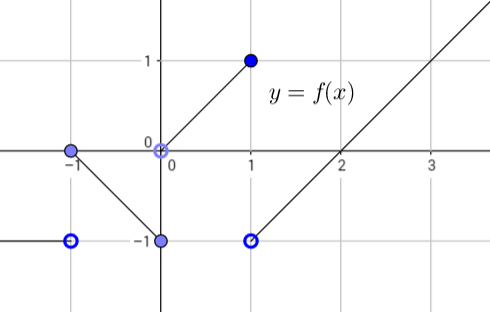
\includegraphics[width=0.4\textwidth]{1}
\end{figure*}
\ans{\(13\)}

%
\prob{}
함수 \(f(x)=\begin{cases}\frac{x^2-ax-2}{x-1}&(x\neq1)\\b&(x=1)\end{cases}\) 실수 전체에서 연속이려면 \(a^2+b^2\)의 값은?
\ans{\(10\)}

\end{document}